\chapter{Problématique et État de l'Art}
\label{ch:problematic}

\section{Introduction}
Ce rapport documente le travail effectué dans le cadre du Travail de Bachelor (TB) de la formation de Sécurité informatique, orientation de la filière Informatique 
et systèmes de communication du département Technologie de l'Information et de la Communication de la HEIG-VD.

Ce projet, intitulé "WiFace" aborde la problématique suivante:

Les dispositifs Wifi diffusent en permanence des trames qui permettent de trouver rapidement les réseaux à
proximité. Ces trames, appelées “probe requests” sont utilisées par des “sniffers” pour “tracer” les utilisateurs dans
des centres commerciaux et d'autres endroits publics.

Ces informations jouissent pourtant d'un certain anonymat. En effet, les adresses MAC des dispositifs sont révélées
par ces trames mais il n'est normalement pas possible de les associer avec l'identité d'un individu. De plus, les
problématiques de « privacy » ont peu à peu amené les constructeurs à implémenter des mécanismes anonymisant
les utilisateurs, par exemple en rendant les adresses MAC pseudo-aléatoires.

Dans ce projet, l'étudiant ou l'étudiante devra concevoir et développer un démonstrateur pour un système capable
de combiner un “sniffer” amélioré capable de récolter les “probe request” et de prendre en même temps des
photos des visages se trouvant à proximité du capteur de trames (par exemple, en face d'une vitrine d'un magasin).
Le système tentera de corréler des adresses MAC et des images de visages récoltées à des endroits différents afin
d'associer un visage à une adresse. Finalement, une recherche par reconnaissance d'images sur les réseaux sociaux
(pour le démonstrateur, la recherche sera faite sur une base de données) essaiera d'obtenir l'identité du
propriétaire du téléphone mobile et toutes les données disponibles sur ce dernier. Des attaques visant la
désanonymisation pourront être mises en place afin de tracer au mieux les utilisateurs.

\section{Démarche et finalité}
Le but recherché est la création d'un \textbf{prototype} en tant que proof of concept afin de démontrer qu'il est facile pour un particulier de mettre un place
une solution de surveillance avec peu de moyen. 

Les conséquences d'un tel constat seront explorées et nous montrerons qu'il n'est peut-être pas souhaitable qu'une telle solution soit disponible sur le marché.  

\section{Travail à effectuer}

En décomposant la problèmatique, plusieurs axes sont mis en évidence:
\begin{enumerate}
\item Développement d'un sniffer de trames Wifi
\item Intégration d'un système de reconnaissance faciale
\item Conception d'un algorithme de couplage Adresse MAC - Image
\item Création d'un prototype embarquant ces technologies sous la forme d'un nano-ordinateur
\item Documentation du travail et création de divers documents techniques (mode d'emploi, étude de marché, ...)
\end{enumerate}

\section{Quelques projets existants}
Une bonne manière de se rendre compte de l'état de l'art est d'explorer divers projets déjà existants.

\subsection{Probe Kit}
\say{A must-have hobby kit for any amateur network data collection}

Probe Kit est un projet développé par Brannon Dorsey et Nick Briz. À la frontière entre technologie et oeuvre d'art, cette initiative nous propose de "collectioner" les
probe requests, sous forme visuelle. 
Ce logiciel sniffe les trames WiFi et établit une liste de probe request par SSID, faisant grandir notre collection au fil du temps.

\begin{figure}[H]
	\centering
	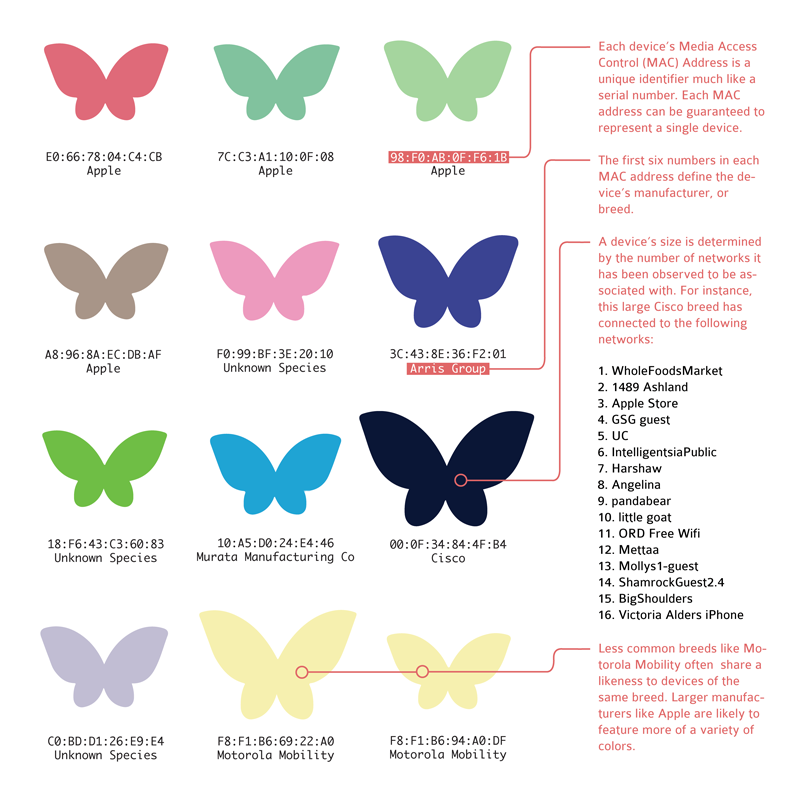
\includegraphics[width=12cm]{images/probekit.png}
	\caption{Démonstration de Probe Kit}
	\label{fig:probekit}
\end{figure}

Avec cette approche ludique, cette démarche vise à sensibiliser les utilisateurs à la recolte passive de données.

\subsection{CrowdProbe}

En plus de la récolte de probe requests, il est possible d'en inférer des données. C'est ce que propose CrowdProbe~\cite{crowdprobe}. 
En installant leur dispositif dans un musée, ils ont réussi à prédire avec une bonne précision le déplacement des utilisateurs, même lors de l'utilisation d'adresse MAC aléatoire.

\begin{figure}[H]
	\centering
	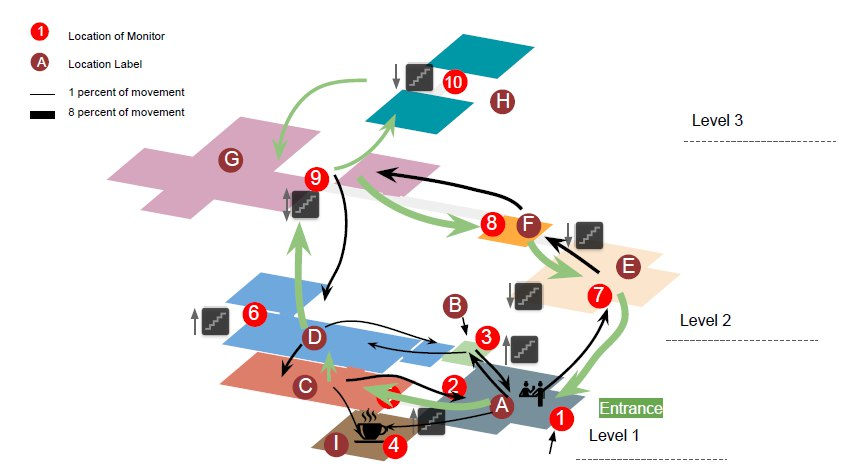
\includegraphics[width=12cm]{images/crowd-probe.jpeg}
	\caption{Flux des visiteurs inféré à l'aide de modèles de Markov}
	\label{fig:crowdprobe}
\end{figure}

\subsection{Serrure déverouillable à l'aide de reconnaissance faciale}
Voici un petit projet~\cite{DOORLOCK} permettant d'utiliser la portabilité de la Raspberry Pi afin de la coupler avec une caméra et une serrure intelligente. 
À l'aide d'OpenCV, le visage de l'utilisateur est reconnu et ouvre la porte si ce dernier est pré-enregistré. 

J'ai inclus ce projet pour montrer qu'il est relativement aisé d'implémenter des mécanismes de reconnaissance faciale à l'aide de la Raspberry Pi
